\chapter{Preparation}

\section{Theory}


\section{Preparation Questions}

\subsection{Question 1}
\begin{figure}[ht]
\centering
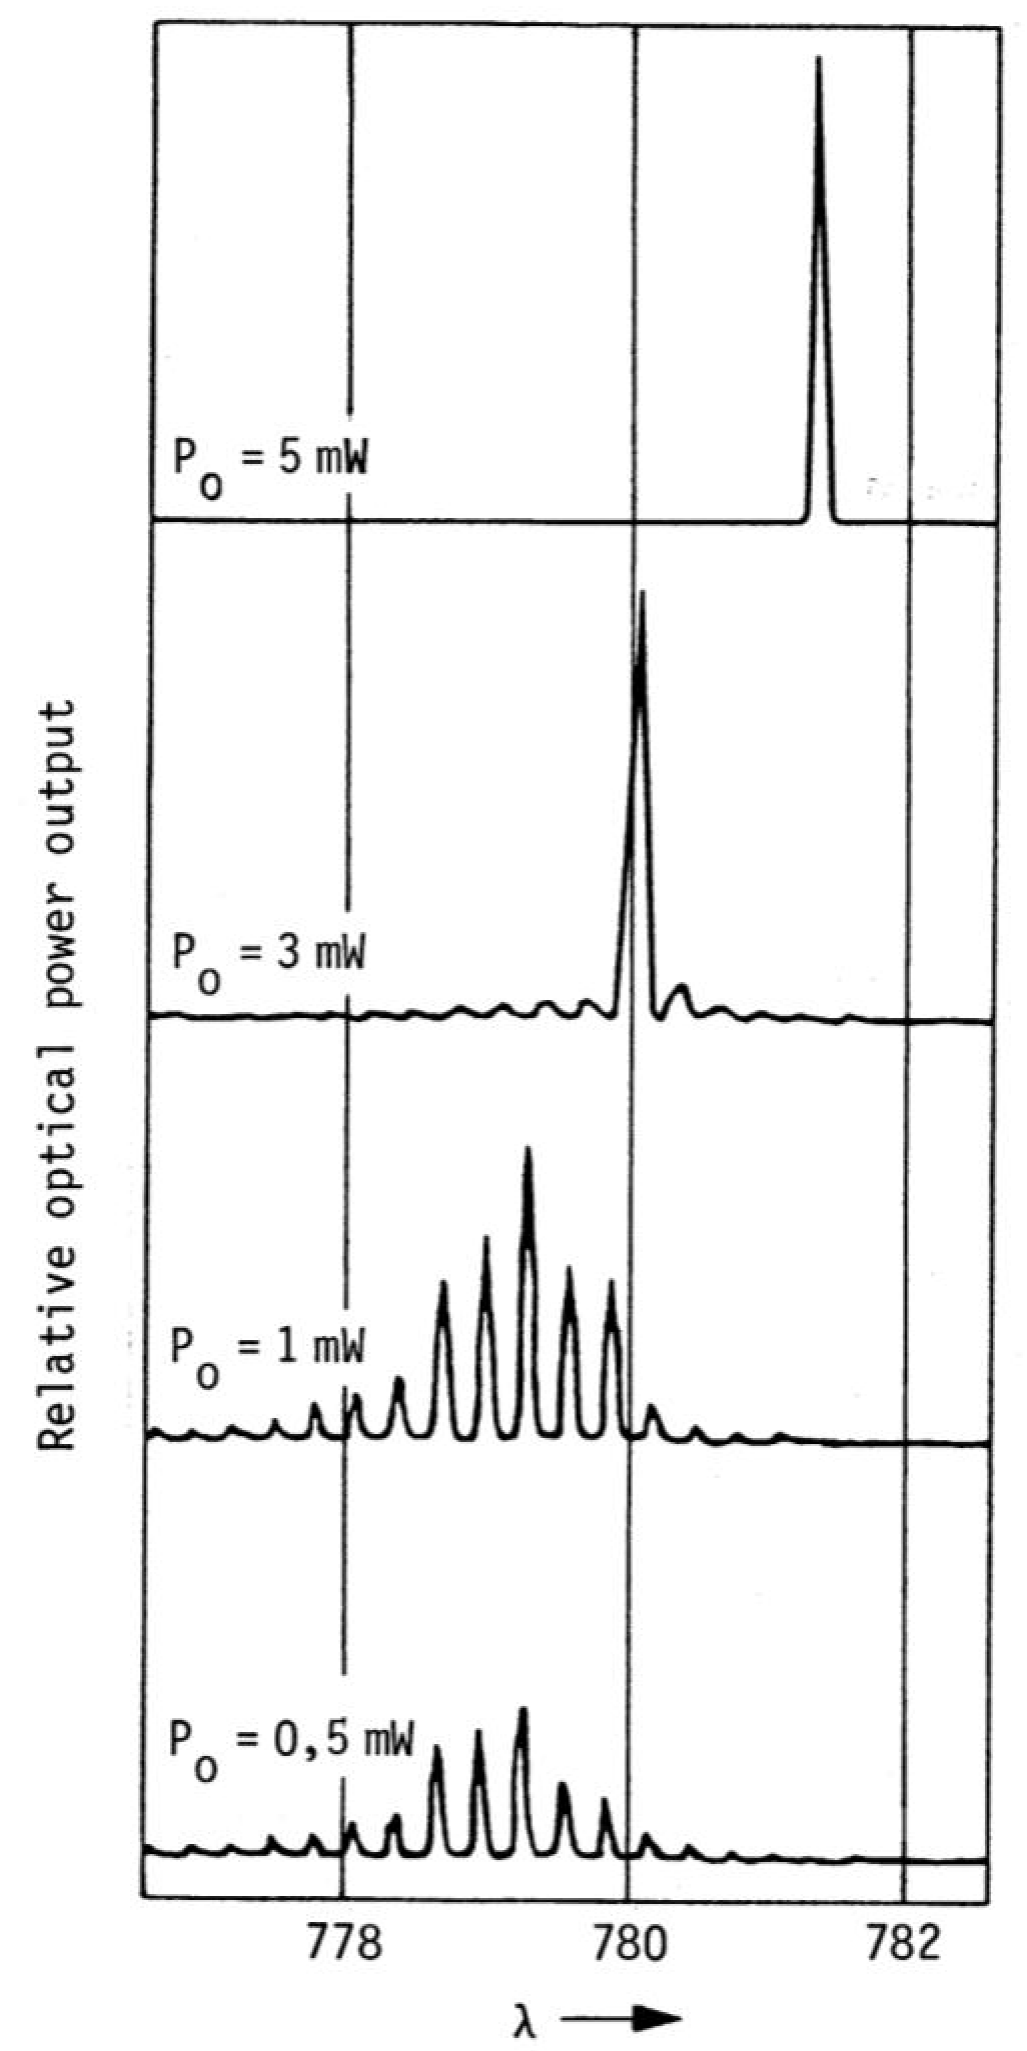
\includegraphics[width=.3\columnwidth]{Grafiken/Q1.png}%
\caption{output spectra of a laser diode for different optical output powers.}%
\label{fig:Q1}%
\end{figure}
Figure \ref{fig:Q1} shows the spectral behaviour of a laser diode at different power levels. At a low power level, there are many intensity peaks. This can be explained by the different modes existing in the laser's resonator. The light generated in the laser diode is only interfering constructively, when the condition
\begin{equation} \frac{n\i{g}\cdot 2L}{\lambda_0} = q \hspace{1,5cm}	 q\in \mathbb{N}	
\end{equation}
is fulfilled, hence only these wavelength are emitted.

Of course this condition holds when the power is increased. However with increasing power the fundamental mode of the resonator is amplified more than the other modes. This can be explained by the fact, that the propability of spontaneous emission into a certain mode increases with the number of photons in that mode. 



% The output spectra of a laser diode is shown in figure \ref{fig:Q1}\footnote[1]{Optical Communications Lab - Experiment 1, Preparation Materials} for different output powers $P_0$. 
% There are different modes in the output spectrum.  How much modes exist depends on the optical gain each mode experiences. For a low output power the the spectrum is multimoded, for a higher power it gets single mode.\footnote[2]{Optoelectronics and Photonics; S. O. Kasap; Prentice Hall, 2001}
% For a low output power several modes can be amplified by the material. For higher powers, all electrons are involved in the amplification of the one mode. The other modes can't be amplified any more.
% \comwo{sehr komische sache, ne quelle wos drinsteht w�r gut}
%  
For higher powers the spectrum of the laser shifts to a longer wavelength.
An applied current through the flows nearly complete through the active zone of the laser diode. Because the refractive index depends on the carrier density\footnote[3]{Optische Nachrichtentechnik; Grau, G.; Freude, W.; 3. ed.; Springer 1991} it changes with higher currents and therefore with higher optical output powers.

Since the resonance frequencies of the laser depend on the refractive index of the material, the frequencies shift with the higher output power as well.

Another explanation could be, that through the higher power the temperature of the laser changes and therefore the frequency shifts. 

\todo{nochmal kontrollieren, und warum �ndert sich der optical gain auch mit der leistung? sicher auch wegen $\Delta n$.}

\subsection{Question 2}
The group refractive index for $\lambda~=~$780~nm in GaAs was ask.
For $n$~=~3.5 and d$n$/d$E$ = 0.4/eV.

\begin{equation}
\begin{split}
n_\mathrm{g} = n - \lambda \frac{\mathrm{d}n}{\mathrm{d}\lambda}\\
\end{split}
\label{eq:}
\end{equation}


with 
\begin{equation}
\begin{split}
\frac{\mathrm{d}E}{\mathrm{d}\lambda}=- \frac{hc}{\lambda^2}\\
\mathrm{d}E=- \frac{hc}{\lambda^2}\mathrm{d}\lambda\\
\end{split}
\label{eq:}
\end{equation}
follows for $\frac{\mathrm{d}n}{\mathrm{d}E}$


\begin{equation}
\begin{split}
\frac{\mathrm{d}n}{\mathrm{d}E}=\frac{0.5}{\mathrm{eV}}=\frac{\mathrm{d}n}{\mathrm{d}\lambda}\frac{-\lambda^2}{hc}\quad.
\end{split}
\label{eq:}
\end{equation}
So $\frac{\mathrm{d}n}{\mathrm{d}\lambda}$ becomes

\begin{equation}
\frac{\mathrm{d}n}{\mathrm{d}\lambda} = \frac{-0.4}{\mathrm{eV}}\frac{hc}{\lambda^2}\quad.
\label{eq:}
\end{equation}

and $n_\mathrm{g}$ can be calculated:

\begin{equation}
\begin{split}
n_\mathrm{g} = n - \lambda\frac{-0.4}{\mathrm{eV}}\frac{hc}{\lambda^2}=4.136 \quad.
\end{split}
\label{eq:ng}
\end{equation}

\subsection{Question 3}

From figure \ref{fig:Q1} the difference of two resonator wavelenth can be estimated. In a range of 2~nm there are 7 peaks. Thus $\Delta\lambda\i{q} \approx \frac{2\mathrm{~nm}}{7} = 0.29$~nm. This corresponds to a frequency difference of 
\begin{equation}
 \left|\Delta f\i{q}\right| = \frac{c\cdot\Delta\lambda\i{q}}{\lambda_0^2} = 138 \mathrm{~GHz} 
\end{equation}
The circulation time in the resonator can be calculated by:
\begin{equation}
 \tau\i{U} = \frac{1}{\Delta f\i{q}} = 7.24\mathrm{~ps}
\end{equation}
With the group velocity form \eqref{eq:ng} the Length the resonator $L$ can be computed by
\begin{equation}
 L = \frac{c\cdot\tau\i{U}}{2n\i{g}} = 262.7 ~\upmu\mathrm{m}
\end{equation}
Expressed in multiples of the resonator wavelength the length of one resonator circulation is:
\begin{equation}
 q = \frac{n\i{g}\cdot 2L}{\lambda_0} = 2786
\end{equation}

\subsection{Question 4}
For perpendicular incident light the power reflection coefficient for a boundary between GaAs and air is given by
\begin{equation}
 R = \left(\frac{n\i{air} - n\i{g}}{n\i{air} + n\i{g}}\right)^2 = 0.373
\label{eq:reflection}
\end{equation}
\comseb{ich bin mir net ganz sicher ob ich $n_g$ oder $n_{GaAs}$ nehmen muss}.

The reflection at the mirrors can also be expressed as an equivalent attenuation or time constant, which is calculated by
\begin{equation}
 \alpha\i{S}=-\frac{\ln R}{L}
\end{equation}
and
\begin{equation}
 \tau\i{R}=\frac{1}{cn\i{g}\alpha\i{S}} 
\end{equation}
respectively.

With the $R$ obtained in \eqref{eq:reflection} this leads to $\alpha\i{S}=0.376\mathrm{~cm}^{-1}$ and $\tau\i{R}=0.215\mathrm{~ps}$. With a attenuation of the medium of about $\alpha\i{V}=40$~cm$^{-1}$ the lifetime of a photon is:
\begin{equation}
 \tau\i{p}=\frac{1}{cn\i{g}(\alpha\i{S}+\alpha\i{V})}= 0.2 \mathrm{~ps}
\end{equation}
This is smaller than the circulation time of the resonator with about a factor 36.
% With this the equivalent attenuation and time constant for the mirrors can be calculated:
% \begin{equation}
%  \alpha\i{S} = 
% \end{equation}


\subsection{Question 5}
\paragraph{5. a)}
\begin{equation}
\frac{\mathrm{d}N\i{p}}{\mathrm{d}t}=N\i{P}\left[ \Gamma G(n\i{T}) - \frac{1}{\tau\i{p}} \right] + \Gamma G(n\i{T})n\i{sp}(n\i{T})
\label{eq:q4a1}
\end{equation}
There are different parts in the differential equation with different physical meanings.\footnote[4]{Lecture Notes: Optical Sources and Detectors; Koos, C.}

\begin{itemize}
	\item $\frac{\mathrm{d}N\i{p}}{\mathrm{d}t}$ is the change of the number of photons per time.
	\item $N\i{P} \Gamma G(n\i{T})$ are the through stimulation generated photons per time.
	\item $-\frac{N\i{P}}{\tau\i{p}}$ are the outcoupled and absorbed photons per time.
	\item $\Gamma G(n\i{T})n\i{sp}(n\i{T})$ are the spontaneously generated photons per mode and time.
\end{itemize}
\comseb{warum: per mode?}
and in

\begin{equation}
\frac{\mathrm{d}(n\i{T} V\i{r})}{\mathrm{d}t} = \frac{I}{e}-r\i{eff}(n\i{T})V\i{R}-N\i{P}\Gamma G(n\i{T})
\label{eq:q4a2}
\end{equation}


\begin{itemize}
	\item $\frac{\mathrm{d}(n\i{T} V\i{r})}{\mathrm{d}t}$ is the change of the number of electrons per time.
	\item $\frac{I}{e}$ are the injected electrons per time
	\item $-r\i{eff}(n\i{T})V\i{R}$ are the spontaneous and non radiative depleted electrons per time.
	\item $-N\i{p}\Gamma G(n\i{T})$ are the through stimulation depleted electrons per time.
\end{itemize}

\todo{Nochmal dr�berschauen, vgl. OWS-Skript: 3.114 (PDF-Seite 117). Daher hab ich die bezeichnungen was was ist. hier sind aber einige elemente leicht anders!!!}
\comseb{bin eigentl zufrieden damit}
\paragraph{5. b)}

At a stationary operatinon point ($N\i{P0}, n\i{T0}$ , $I_0$) equation \eqref{eq:q4a1} and \eqref{eq:q4a2} can be simplified to

\begin{equation}
0 = N\i{P}\left[\Gamma G(n\i{T0})- \frac{1}{\tau\i{P}}\right] +\Gamma G(n\i{T})n\i{sp}(n\i{T})
\label{eq:dgl_stat1}
\end{equation}
and
\begin{equation}
 0 = \frac{I\i{0}}{e}-r\i{eff}(n\i{T0})V\i{R}-N\i{P}\Gamma G(n\i{T0}),
\label{eq:dgl_stat2}
\end{equation}
respectively.

The number of emitted photons at the operation point $N\i{P0}$ can be obtained by rearranging \eqref{eq:dgl_stat1} to:
\begin{equation}
N\i{P0}=\tau\i{P}\left(\frac{I_0}{e}-r\i{eff}(n\i{T0})V\i{R}\right).
\label{eq:}
\end{equation}
For
\begin{equation}
 I_0 \gg er\i{eff}(n\i{Ts})V\i{R}
\end{equation}
% i.e. there are much more electrons generated, than there are spontaniously recombining, the term $\Gamma G(n\i{T})n\i{sp}(n\i{T})$ in \eqref{eq:dgl_stat2} can be neglected as well. Thus $\Gamma G(n\i{T0})$ and $N\i{P0}$ can be calculated by:
 i.e. the current $I_0$ is much bigger than the threshold current of the laser, the spontaneous emission in \eqref{eq:dgl_stat2} can be neglected as well. Thus $\Gamma G(n\i{T0})$ and $N\i{P0}$ can be calculated by:

\begin{equation}
\Gamma G(n\i{T0}) = \frac{1}{\tau\i{P}}
\label{eq:}
\end{equation}
\begin{equation}
N\i{P0}=\tau\i{P}\cdot\frac{I_0}{e}
\label{eq:}
\end{equation}


% 
% 
% %%%%%%
% With this equations both $\Gamma G(n\i{T0})$ and $N\i{P0}$ can be calculated.
% 
% \begin{equation}
% \Gamma G(n\i{T0}) = \frac{1}{\tau\i{P}}
% \label{eq:}
% \end{equation}
% \begin{equation}
% N\i{P0}=\tau\i{P}\left(\frac{I_0}{e}-r\i{eff}(n\i{T0})V\i{R}\right)
% \label{eq:}
% \end{equation}
% 
% For $I_0 > er\i{eff}(n\i{Ts})V\i{R}$ $N\i{P}$ is positive and therefore useful. Here more Photons are generated then photons are lost.
% 
% \todo{Ich habe die Frage nicht verstanden "`F�r welche Laserstr�me ist diese Voraussetzung am besten erf�llt"'? vgl. auch OWS-Script "`Lasing threshold"' Pdf Seite 118}


\paragraph{5. c)}
The frequency response of the diode
\begin{equation}
H\i{Kl}(f)=\frac{\omega\i{r}^2}{(\mathrm{j}\omega)^2 + 2\gamma\i{r}(\mathrm{j}\omega)+\omega\i{r}^2}
\label{eq:freq_resp}
\end{equation}
leads to $H\i{Kl}(0)=1$ and thereby
\begin{equation}
\left|\frac{H\i{Kl}(f\i{Kl})}{H\i{Kl}(0)}\right| = \left|H\i{Kl}(f\i{Kl})\right|
\label{eq:}
\end{equation}
\begin{equation}
|H\i{Kl}(f\i{Kl})|=\frac{|\omega\i{r}^2|}{|(\mathrm{j}\omega\i{Kl})^2 + 2\gamma\i{r}(\mathrm{j}\omega\i{Kl})+\omega\i{r}^2|}=\frac{\omega\i{r}^2}{\sqrt{(\omega\i{r}^2+\omega\i{Kl}^2)^2 + (2\gamma\i{r}\omega\i{Kl})^2}}
\label{eq:}
\end{equation}

This needs to be maximized:
\begin{equation}
\begin{split}
\frac{\mathrm{d}|H\i{Kl}(f\i{Kl})|}{\mathrm{d}\omega\i{Kl}}=0\\
=\frac{\omega\i{r}^2 (4\omega\i{r}^2\omega\i{Kl}+4\omega\i{Kl}^3+8\omega\i{Kl}\gamma\i{r}) }{2(\omega\i{r}^4 + 2\omega\i{r}^2\omega\i{Kl}^2+\omega\i{Kl}^4+4\omega\i{Kl}^2\gamma\i{r}^2)^{\frac{3}{2}}}\\
4\omega\i{r}^2\omega\i{Kl}+4\omega\i{Kl}^3+8\omega\i{Kl}\gamma\i{r}=0
\end{split}
\label{eq:}
\end{equation}
this leads to

\begin{equation}
\omega\i{Kl} = \sqrt{-\omega\i{r}^2-2\gamma\i{r}^2}
\label{eq:}
\end{equation}

There must be an error in the derivation of this term. After source \footnote[3]{Optische Nachrichtentechnik; Grau, G.; Freude, W.; 3. ed.; Springer 1991} the correct soultion should be

$\omega\i{Kl}=\sqrt{\omega\i{r}^2 - 2\gamma\i{r}^2}$.

For operation of the laser beneath threshold \eqref{eq:freq_resp} is invalid. In that domain, there is no stimulated emmission and thus no spontaneous emmision has to be taken into account. 
% 
% Driving the laser below the threshold  means, that there is no stimulated emission. Only spontaneous emission could be taken into account. 
% 
% \todo{nochmal �berlegen was da so passiert}

\paragraph{5. d)}
Starting from 
\begin{equation}
\omega\i{r}^2 = \frac{1}{\tau\i{P}}\frac{\Gamma N\i{P0}}{V\i{R}}\frac{\partial G}{\partial n\i{T}}
\label{eq:}
\end{equation}

and using
\begin{equation}
\begin{split}
\frac{\Gamma \partial G}{\partial n\i{T}} =\frac{G(n\i{t})}{r\i{eff}(n\i{T})\tau\i{eff}}\quad,\\
\frac{N\i{P0}}{\tau\i{P}}= \frac{I-I\i{s}}{e} \quad\mathrm{and}\\
G(n\i{t})=\frac{1}{\tau\i{P}}
\end{split}
\label{eq:}
\end{equation}
leads to
\begin{equation}
\omega\i{r}^2 = \frac{I-I\i{s}}{e\tau\i{P} V\i{R}r\i{eff}\tau\i{eff}}
\label{eq:}
\end{equation}
and simplifies with
\begin{equation}
I\i{s}=er\i{eff}(n\i{TS})V\i{R} \quad \mathrm{and}
\label{eq:}
\end{equation}

to 
\begin{equation}
\omega\i{r}^2 = \frac{1}{\tau\i{P}\tau\i{eff}}\left(\frac{I_0}{I\i{S}}-1\right)\quad.
\label{eq:}
\end{equation}

Using the same simplifications as before the following can be derivated:
\begin{equation}
2\gamma\i{r}=\frac{1}{\tau\i{eff}}\frac{I_0}{I\i{S}}\quad.
\label{eq:}
\end{equation}

\subsection{Question 6}
\paragraph{6. a)}
``The attenuation of the relaxation oscillation is dominated by the spontaneous emission in the range of the threshold.''\footnote[3]{Optische Nachrichtentechnik; Grau, G.; Freude, W.; 3. ed.; Springer 1991}
\paragraph{6. b)}
